\documentclass{beamer}

\usepackage{ucs}
\usepackage[utf8x]{inputenc}
\usepackage[T1]{fontenc}
\usepackage[english]{babel}
\usepackage{epstopdf}

%\usepackage{multirow}%	multirow
%\usepackage[retainorgcmds]{IEEEtrantools}%	IEEEeqnarray
%\usepackage{mathabx}%	convolution symbol
\usepackage{relsize}%	relative font sizes
%\usepackage{listings}
%\usepackage{graphicx}


%	presentation info
\title{OpenMP analysis}
\subtitle{A finite volume case study from an industrial application}

\author{M. Palhas \and P. Costa}

\institute[19808 \and 19830]{
	University of Minho\\
	Department of Informatics
}

\date{Braga, March 2012}


%	beamer options
\usetheme{CambridgeUS}


\begin{document}%	begin presentation

\maketitle%	title slide

%\begin{frame}
%	\frametitle{Index}
%	\tableofcontents
%\end{frame}

\begin{frame}
	\frametitle{Parallelization}
	\begin{figure}
		\begin{center}
			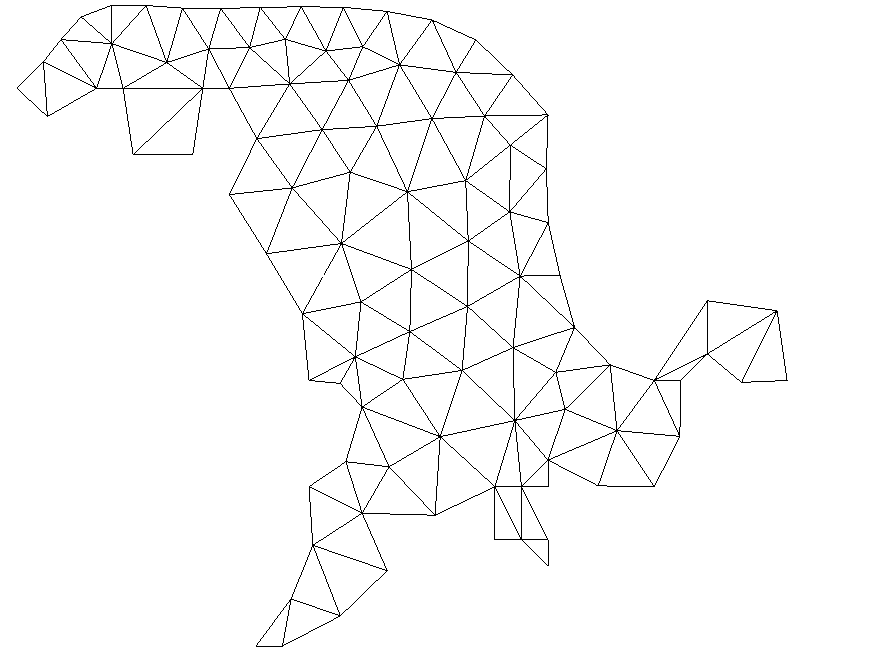
\includegraphics[height=0.8\textheight]{images/slides.march/mesh0.png}
		\end{center}
	\end{figure}
\end{frame}

\begin{frame}
	\frametitle{Algorithm}
	\begin{itemize}
		\item{Heartbeat algorithm:
		\begin{enumerate}
			\item{Compute the pollution fluxes;}
			\item{Update the pollution levels;}
		\end{enumerate}
		}
		\item{\texttt{compute\_flux}
		\begin{itemize}
			\item{Iterate over \textbf{edges};}
			\item{Dependency when calculating $\delta t$
			\begin{itemize}
				\item{Removed replacing with a sum reduction;}
				\item{Implementation simplifications allow to remove this completely;}
			\end{itemize}
			}
		\end{itemize}
		}
		\item{\texttt{update}
		\begin{itemize}
			\item{Originally iterate over \textbf{edges};}
			\item{Race condition in \textbf{cells};
			\begin{itemize}
				\item{Removed changing to cell iterations;}
				\item{Hurts locality;}
			\end{itemize}
			}
		\end{itemize}
		}
	\end{itemize}
\end{frame}

\begin{frame}
	\frametitle{Computational Intensity}
	\begin{minipage}{0.78\textwidth}
		\begin{figure}
			\begin{center}
				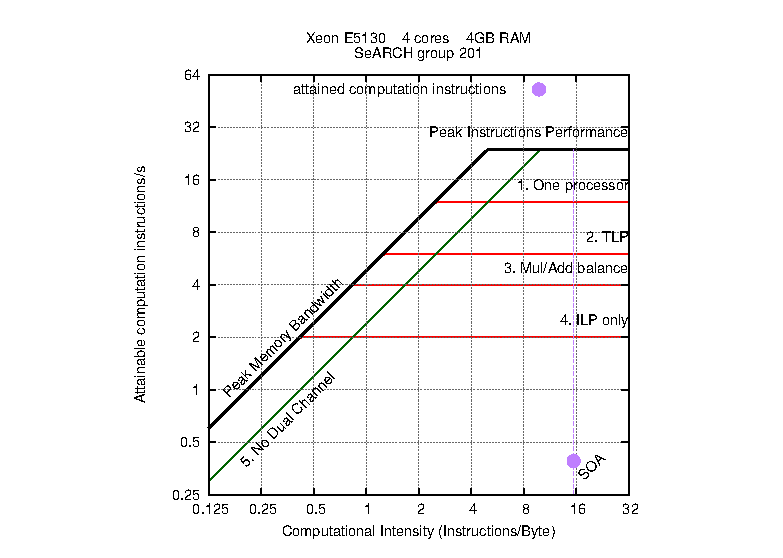
\includegraphics[width=\textwidth]{images/roofline/201.eps}
			\end{center}
		\end{figure}
	\end{minipage}
	\begin{minipage}{0.2\textwidth}
		\begin{itemize}
			\item[(3)]{medium}
			\item[(4)]{big}
			\item[(5)]{huge}
		\end{itemize}
	\end{minipage}
\end{frame}

\begin{frame}
	\frametitle{Instruction Mix}
	\begin{figure}
		\begin{center}
			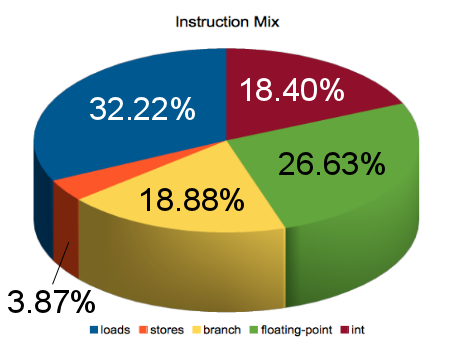
\includegraphics[width=0.6\textwidth]{images/slides.march/instmx.png}
		\end{center}
	\end{figure}
\end{frame}

\section{Granularity}
\begin{frame}
	\frametitle{Step Time}
	\begin{figure}
		\begin{center}
			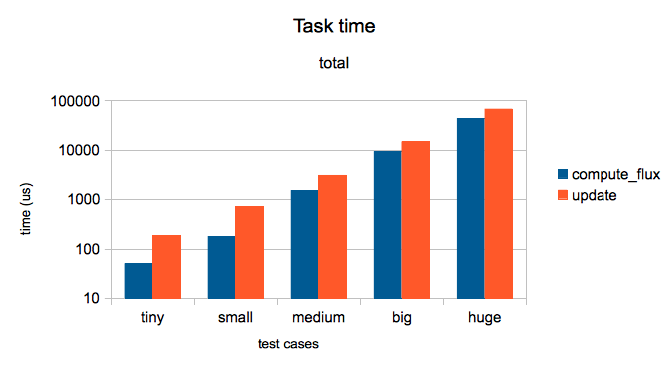
\includegraphics[width=\textwidth]{images/slides.march/tasktime_total.png}
		\end{center}
	\end{figure}
\end{frame}

\section{Task balance}
\begin{frame}
	\frametitle{Action Time}
	\begin{figure}
		\begin{center}
			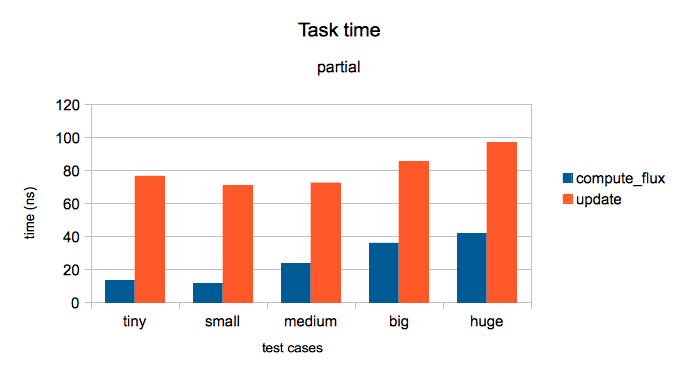
\includegraphics[width=\textwidth]{images/slides.march/tasktime_partial.png}
		\end{center}
	\end{figure}
\end{frame}

\section{Conclusions}
\begin{frame}
	\frametitle{Conclusions}
	\begin{itemize}
		\item{Memory bound implementation;}
		\item{Locality improvements are possible, but may be limited;}
		\item{Parallelizable tasks total time significantly greater than the OpenMP overhead;
			\begin{description}
				\item[\texttt{PARALLEL FOR}]{--- 2.85 $\mu$s overhead}
			\end{description}
		}
		\item{Synchronization only between the heartbeat phases;}
		\item{The program is \textbf{heterogeneous};
		\begin{itemize}
			\item{\texttt{update} > \texttt{compute\_flux}}
		\end{itemize}
		}
		\item{Each task is \textbf{homogeneous};}
	\end{itemize}
\end{frame}

\section{Questions}
\begin{frame}
	\titlepage
	\begin{center}
		\Huge\bfseries
		- ? -
	\end{center}
\end{frame}

\end{document}%	end presentation
